\documentclass[journal, a4paper]{IEEEtran}

\usepackage[section]{placeins}
\usepackage{graphicx} 
\usepackage{url}      
\usepackage{amsmath}
  \begin{document}
	\title{Deep Neural Network}
	\author{Group - 11,
		\\School of Engineering and Applied Science,\\
		Ahmedabad University,\\ Courses : Machine Learning, Algorithms and Optimization for Big Data\\
		\textbf{Working Group:} Madhav Chavda, Ravi Patel, Jayveer Gadhvi, Jay Dangar
	}

	\maketitle
\begin{abstract}
	In this paper, we provided an overview of the Deep Neural Network(DNN). We know that we can process on data using different algorithm as we want, but for that we need to implement an algorithm. But instead of that we can design a machine which can observe the process which we do on the input data and generate a way to do that processs by itself. We implemented an small neural network and tasted using inputing the dataset. And that neural network works as we have implented. \\
	Index Terms \textendash Neural Network, Deep Neural Network.
\end{abstract}


\section{Defination and Application}
	\PARstart{D}{eep} learning is a class of machine learning that use a cascade of many layer of nonlinear processing units for feature extraction and transformation. Each successive layer uses the output from the previous layer as input.\\In a simpler way Neural Networks are set of a algorithms, modeled loosely afte the human brain, that are designed to recognize patterns\\Neural networks extract features that are fed to other algorithms for clustering and classification; so you can think of deep neural networks as components of larger machine-learning applications involving algorithms for reinforcement learning, classification and regression.\\Application of the deep neural network are as follow:
	
	\begin{itemize}
	
	\item Detect faces, identify people in images, recognize facial expressions (angry, joyful)
	
	\item Identify objects in images (stop signs, pedestrians, lane markers…)
	
	\item Detect voices, identify speakers, transcribe speech to text, recognize sentiment in voices
	
	\item Classify text as spam (in emails); recognize sentiment in text (customer feedback)
	
	\end{itemize}
	
	Any labels that humans can generate, any outcomes you care about and which correlate to data, can be used to train a neural network. 
	
\section{Key concept and Elements}
	Neural Network composed of several layers. The layers are mande of nodes. A node is just a place where computation happens. A node combines input from the data with a set of coefficients, or weights, that either amplify that input, thereby assigning significance to inputs for the task the algorithm is trying to learn. These input-weight products are summed and the sum is passed through a nodes to determine whether and to what extent that signal progresses further.\\Deep-learning networks are distinguished from the more commonplace single-hidden-layer neural networks by their depth; that is, the number of node layers through which data passes in a multistep process of pattern recognition.
	
	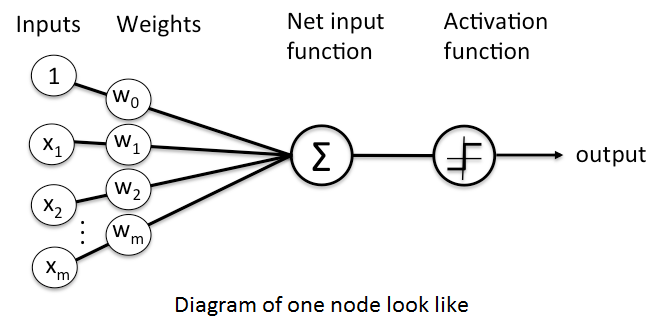
\includegraphics[scale=0.4]{first.PNG}

\FloatBarrier
\section{Application of Deep Neural Network}
	In our Example, we are taking dataset of images of different kind of hand written numbers and giving them as input matrix to the neurons for learning and through learning we are predicting the accuracy of the output predicted by our neuron network. 
		
	\begin{figure}[h]
    	\centering
    	\textbf{Output}\par\medskip
    	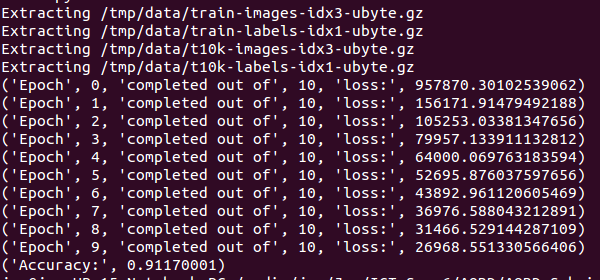
\includegraphics[scale=0.3]{Output.png}
    	\caption{This Figure shows the Accuracy of the learning algorithm.}
	\end{figure}
	
	In, our Example the accuracy given by our neuron network is 0.91 and this is because data to be taken at a time is 1000 and if we decrese this rate of taking input at a time than accuracy will increases.
	
\section{Conclusion}
	

% Now we need a bibliography:
\begin{thebibliography}{9}
	\bibitem{1}
	https://www.tensorflow.org
	\bibitem{2}
	http://neuralnetworksanddeeplearning.com
	\bibitem{3}
	Machine Learning with Python youtube channel by sentdex
	\bibitem{4}
	For Understanding concept of Neural Network, The Course on Machine Learning by Andrew Ng on coursera. 
		
		
\end{thebibliography}



% Your document ends here!
\end{document}